\subsection{XAI-Plattformen}
\todo[inline]{Ich überlege noch wie/ob ich einen Unterschied zwischen Visualisierungstools, Plattformen, Toolkits mache}
Zur Unterstützung bei der Anwendung von XAI-Methoden können Plattformen genutzt werden.

Für das Entwickeln von Plattformen haben \cite{rajabiyazdi2020machine} einige Charakteristiken identifiziert, welche optimalerweise vorhanden sein müssen. Zunächst wird auf die \emph{Mensch-Maschinen-Interaktion} eingegangen. In einer Benutzeroberfläche sollten kontextbezogene Informationen neben Gründen für eine Vorhersage vorhanden sein. Daneben sollte auch eine Darstellung über den Entwicklungsprozess vorhanden sein. \emph{Entscheidungsfindung} sollte durch eine Plattform auch unterstützt werden. Bei Entscheidungsunterstützungen sollte auch in der Plattform beachtet werden, dass diese den Plänen der Organisation folgen sollten. Daneben sollte der Prozess Entscheidungsfindung auch das Fachwissen der Nutzer unterstützen. Das Tool sollte außerdem Risiken aufzeigen, welcher mit einer Entscheidung, die auf Grundlage des Outputs getroffen werden einhergehen. Die \emph{Architektur} eines Systems ist im Idealfall in einer Plattform zu zeigen. Inhalte, die in Bezug auf die Architektur erfasst werden sollten sind z.B. die Datenerfassung, die Datenanalyse, oder das Bewerten von Prognosen. Auch Informationen anderer Systeme sollten integriert werden. Kommt es zu Ausfällen bei Prognosen, hat die Plattform auf diese aufmerksam zu machen. \cite{rajabiyazdi2020machine} haben selbst eine experimentelle Plattform vorgestellt, welche als Automated Reliability Decision Aid System (ARDAS) bezeichnet wird.

Zum Anwenden verschiedener XAI-Methoden existieren Software-Toolkits. Ein Beispiel ist das AI Explainability 360 Toolkit von IBM \footnote{https://aix360.mybluemix.net/} \cite{arya2021ai}. Dieses Toolkit unterstützt die Entwicklung von ML-Algorithmen in der Programmiersprache Python mithilfe von acht verschiedenen Erklärungsmethoden:
\begin{itemize}
    \item \emph{Boolean Decision Rules via Column Generation} werden mithilfe des BRCGExplainer erklärt, welcher binäre Klassifikation unterstützt und direkt interpretierbar ist \cite{dash2018boolean}
    \item Die direkt interpretierbaren \emph{Generalized Linear Rule Models} werden mithilfe des GLRMExplainer erklärt \cite{wei2019generalized}
    \item Der \emph{ProtodashExplainer} ist für das Erläutern von Datensätzen zuständig. Hier werden repräsentative Teile der Daten ausgewählt oder Testinstanzen erklärt \cite{gurumoorthy2019efficient}.
    \item Der \emph{ProfWeightExplainer} liefert globale Erklärungen durch das Darstellen von Gewichten neuronaler Netze \cite{dhurandhar2018improving}.
    \item Personenspezifische Erklärungen werden mithilfe des \emph{TEDExplainers} umgesetzt \cite{hind2019ted}.
    \item Die Methode von \cite{dhurandhar2018explanations} (\emph{CEMExplainer}) wird genutzt, um lokale Erklärungen zu generieren. Dies sind konstrative Erklärungen. Z.B. wird die Frage beantwortet, was minimal ausreichend ist, um die ursprüngliche Klassenvorhersage beizubehalten.
    \item Für Erklärungen von Bildern wird der \emph{CEMMAFImageExplainer} nach \cite{luss2019generating} eingesetzt.
    \item Abhängigkeiten von Merkmalen werden mithilfe von dem \emph{IPVAEExplainer} nach \cite{kumar2017variational} verdeutlicht.
\end{itemize}
Daneben bietet das Explainability 360 Toolkit auch Bewertungsmetriken an und eine erweiterbare Softwarearchitektur. \cite{arya2021ai} empfehlen für das Arbeiten mit ihrem Toolkit des Weiteren einen drei-schrittigen Ablauf, welcher zunächst das Filtern auf verschiedene Instanzen vorsieht. Daraufhin sollten Merkmale einzelner Instanzen präsentiert werden und diese sollten mit anderen Instanzen verglichen werden. Abschließend sollten Ekrlärungen generiert werden, z.B. kontrafaktische Erklärungen. Auch \cite{arya2021ai} weisen darauf hin, dass es schwierig ist zu entscheiden, welche Erklärung genau zu wählen ist. Zielgruppe dieses Tookits sind Entwickler und Data Scientists. Zur Unterstützung werden außerdem Tutorials angeboten, welche auch mit fachlichem Kontext (Medizin) vorhanden sind.
\begin{figure}[h]
    \centering
    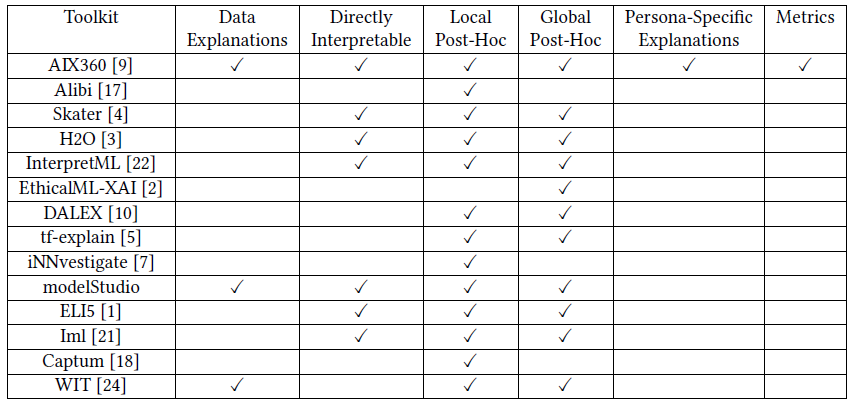
\includegraphics[scale=0.6]{pic/MA-Bilder/Literaturrecherche/30-Toolkits.PNG}
    \caption{Toolkits im Vergleich, entommen aus: \cite{arya2021ai}}
    \label{Fig:toolkitsvergleich}
\end{figure}

Neben dem Explainability 360 Toolkit weisen \cite{arya2021ai} auch auf andere Toolkits hin und vergleichen diese in Abbildung \ref{Fig:toolkitsvergleich} in Bezug auf ihre Funktionalitäten.